\documentclass[border=10pt]{standalone}
\usepackage{tikz}
\usetikzlibrary{arrows.meta, fit, backgrounds, positioning, calc}
\usepackage{amsmath, amssymb}

%% ─── colour palette ───────────────────────────────────────────────────────────
\definecolor{Cteacher}{RGB}{41,98,255}      % blue
\definecolor{Cpursue} {RGB}{0,150,108}      % teal/green
\definecolor{Cevbmf}  {RGB}{230,120,20}     % orange
\definecolor{Ctrain}  {RGB}{120,40,180}     % purple
\definecolor{Cout}    {RGB}{200,30,50}      % red

\begin{document}
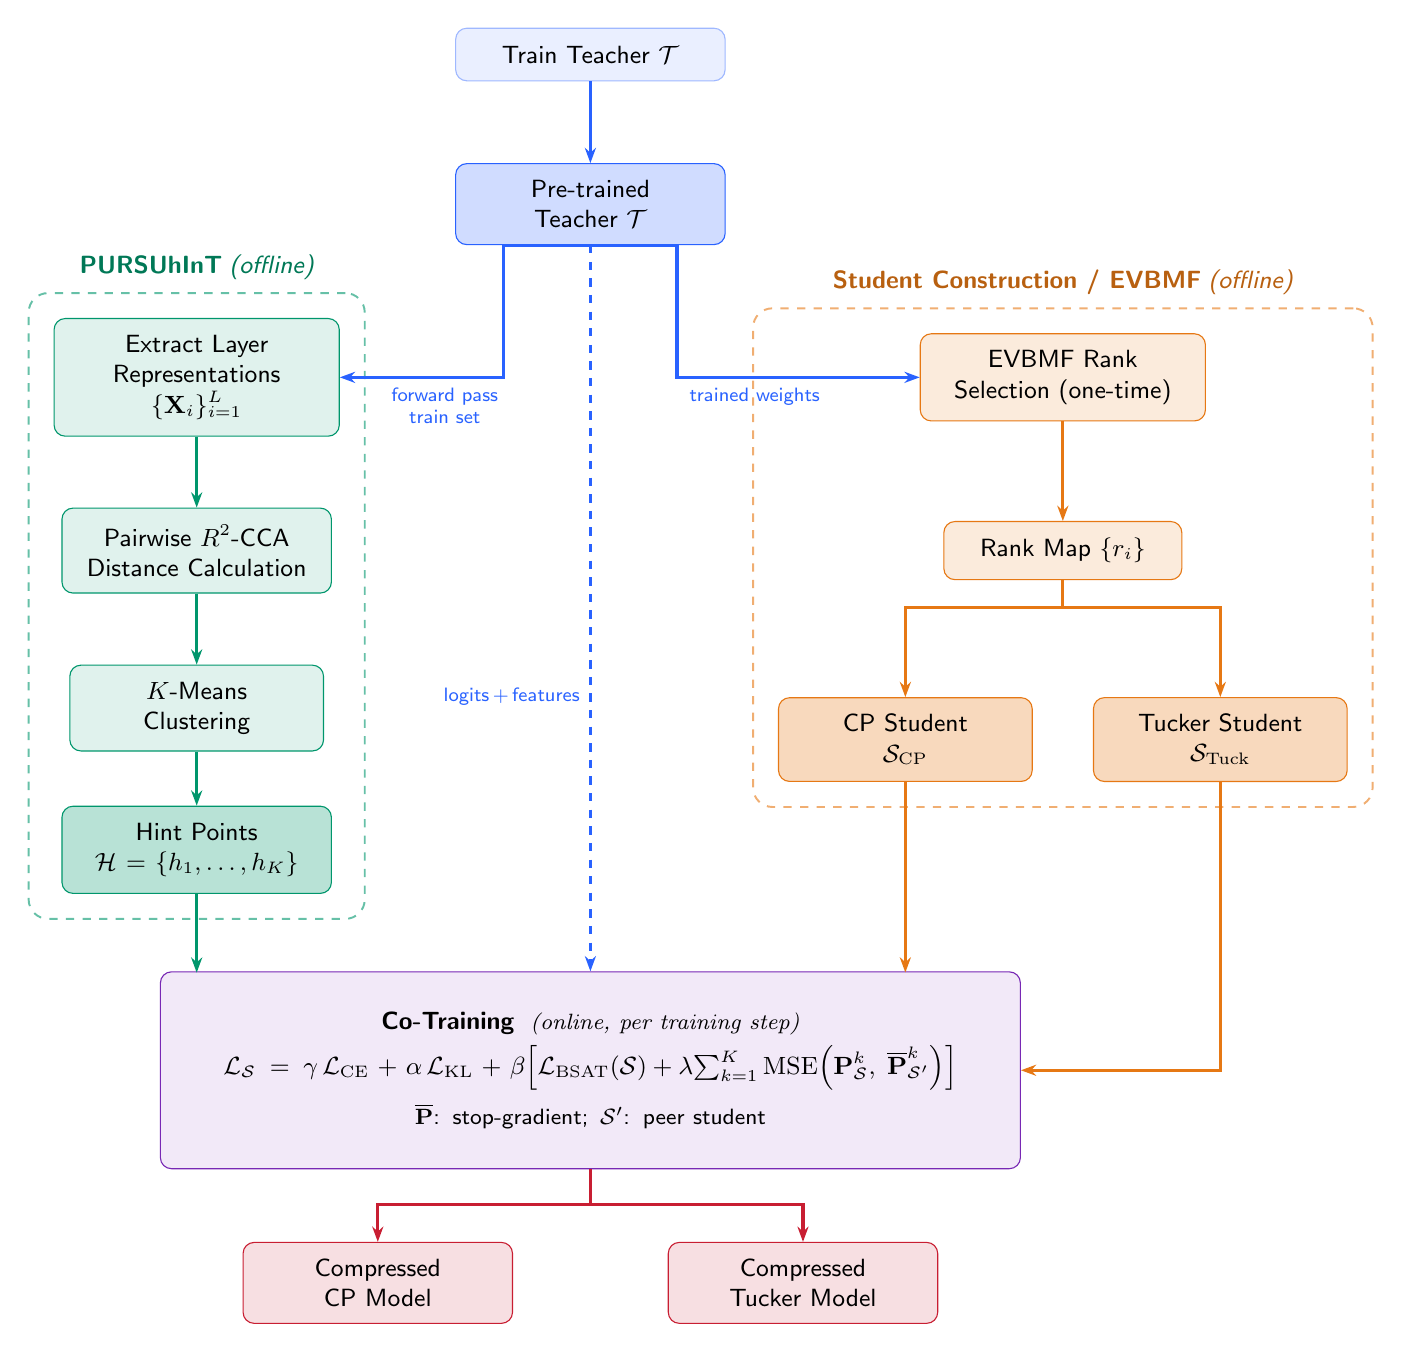
\begin{tikzpicture}[
  font=\small\sffamily,
  box/.style={draw, rounded corners=4pt, align=center,
              inner sep=6pt, minimum height=1.9em},
  grp/.style={draw, dashed, rounded corners=7pt,
              inner sep=9pt, line width=0.7pt},
  A/.style={-{Stealth[length=5.5pt,width=4pt]}, line width=1.1pt, #1},
]

%% ══════════════════════════════════════════════════════════════════════════════
%%  STAGE 0 — Teacher pre-training  (top)
%% ══════════════════════════════════════════════════════════════════════════════
\node[box, fill=Cteacher!10, draw=Cteacher!45, text width=3cm] (Ttrain)
  at (6.5, 1.9)
  {Train Teacher $\mathcal{T}$};

\node[box, fill=Cteacher!22, draw=Cteacher, text width=3cm] (T)
  at (6.5, 0)
  {Pre-trained\\Teacher $\mathcal{T}$};

\draw[A=Cteacher] (Ttrain) -- (T);

%% ══════════════════════════════════════════════════════════════════════════════
%%  PURSUhInT  (left column)                             [OFFLINE]
%% ══════════════════════════════════════════════════════════════════════════════
\node[box, fill=Cpursue!12, draw=Cpursue, text width=3.2cm] (ext)
  at (1.5, -2.2)
  {Extract Layer\\Representations\\$\{\mathbf{X}_i\}_{i=1}^{L}$};

\node[box, fill=Cpursue!12, draw=Cpursue, text width=3cm] (cca)
  at (1.5, -4.4)
  {Pairwise $R^2$-CCA\\Distance Calculation};

\node[box, fill=Cpursue!12, draw=Cpursue, text width=2.8cm] (km)
  at (1.5, -6.4)
  {$K$-Means\\Clustering};

%% FIXED: was {h_1,h_2,h_3} — methodology uses generic K throughout
\node[box, fill=Cpursue!28, draw=Cpursue, text width=3cm] (H)
  at (1.5, -8.2)
  {Hint Points\\$\mathcal{H}=\{h_1,\ldots,h_K\}$};

%% ══════════════════════════════════════════════════════════════════════════════
%%  STUDENT CONSTRUCTION (EVBMF)  (right column)         [OFFLINE]
%% ══════════════════════════════════════════════════════════════════════════════
\node[box, fill=Cevbmf!15, draw=Cevbmf, text width=3.2cm] (evbmf)
  at (12.5, -2.2)
  {EVBMF Rank\\Selection (one-time)};

\node[box, fill=Cevbmf!15, draw=Cevbmf, text width=2.6cm] (rmap)
  at (12.5, -4.4)
  {Rank Map $\{r_i\}$};

\node[box, fill=Cevbmf!28, draw=Cevbmf, text width=2.8cm] (cp)
  at (10.5, -6.8)
  {CP Student\\ $\mathcal{S}_{\mathrm{CP}}$};

\node[box, fill=Cevbmf!28, draw=Cevbmf, text width=2.8cm] (tuck)
  at (14.5, -6.8)
  {Tucker Student\\ $\mathcal{S}_{\mathrm{Tuck}}$};

%% ══════════════════════════════════════════════════════════════════════════════
%%  CO-TRAINING  (wide box)                              [ONLINE]
%%
%%  FIXED equation:
%%    • subscript L_S (per-student, not shared)
%%    • sum over k=1..K (not h∈H)
%%    • projectors carry hint-point index k
%%    • \bar{P} denotes stop-gradient (matches methodology notation)
%%    • footnote clarifies notation; removes ambiguous "bidirectional" claim
%% ══════════════════════════════════════════════════════════════════════════════
\node[box, fill=Ctrain!10, draw=Ctrain, text width=10.5cm,
      minimum height=2.5cm] (train)
  at (6.5, -11)
  {\textbf{Co-Training}
   \;{\footnotesize\normalfont\itshape(online, per training step)}\\[3pt]
   $\mathcal{L}_{\mathcal{S}} =
     \gamma\,\mathcal{L}_{\mathrm{CE}}
     + \alpha\,\mathcal{L}_{\mathrm{KL}}
     + \beta\!\left[\mathcal{L}_{\mathrm{BSAT}}(\mathcal{S})
       + \lambda\!\sum_{k=1}^{K}
         \operatorname{MSE}\!\left(
           \mathbf{P}_{\mathcal{S}}^{k},\;
           \overline{\mathbf{P}}_{\mathcal{S}'}^{k}
         \right)\right]$\\[4pt]
   {\footnotesize
    $\overline{\mathbf{P}}$: stop-gradient;\enspace
    $\mathcal{S}'$: peer student}};


%% ══════════════════════════════════════════════════════════════════════════════
%%  OUTPUTS
%% ══════════════════════════════════════════════════════════════════════════════
\node[box, fill=Cout!14, draw=Cout, text width=3cm] (ocp)
  at (3.8, -13.7)
  {Compressed\\CP Model};

\node[box, fill=Cout!14, draw=Cout, text width=3cm] (otk)
  at (9.2, -13.7)
  {Compressed\\Tucker Model};

%% ══════════════════════════════════════════════════════════════════════════════
%%  ARROWS
%% ══════════════════════════════════════════════════════════════════════════════

%% Teacher → PURSUhInT
\draw[A=Cteacher] (T.south) -- +(-1.1,0) |- (ext.east)
  node[pos=0.68, below, font=\scriptsize\sffamily, Cteacher,
     align=center, text width=1.8cm]{forward pass\\ train set};



%% Teacher → EVBMF
\draw[A=Cteacher] (T.south) -- +(1.1,0) |- (evbmf.west)
  node[pos=0.66, below, font=\scriptsize\sffamily, Cteacher]
  {trained weights};

%% PURSUhInT chain
\draw[A=Cpursue] (ext) -- (cca);
\draw[A=Cpursue] (cca) -- (km);
\draw[A=Cpursue] (km)  -- (H);

%% EVBMF chain → students
\draw[A=Cevbmf] (evbmf) -- (rmap);
\draw[A=Cevbmf] (rmap.south) -- +(0,-0.35) -| (cp.north);
\draw[A=Cevbmf] (rmap.south) -- +(0,-0.35) -| (tuck.north);

%% Hint points → co-training
\draw[A=Cpursue] (H.south) -- +(0,-1.0);

%% Students → co-training
\draw[A=Cevbmf] (cp.south) -- +(0,-2.42);
\draw[A=Cevbmf] (tuck.south) -- +(0,-0.5) |- (train.east);

%% Teacher → co-training (frozen inference; dashed)
\draw[A=Cteacher, dashed]
  (T.south) -- +(0,-0.5) -| (train.north)
  node[pos=0.8, left, font=\scriptsize\sffamily, Cteacher]
  {logits\,+\,features};

%% Outputs
\draw[A=Cout] (train.south) -- +(0,-0.45) -| (ocp.north);
\draw[A=Cout] (train.south) -- +(0,-0.45) -| (otk.north);

%% ══════════════════════════════════════════════════════════════════════════════
%%  GROUP BORDERS  (labels now include phase annotation)
%% ══════════════════════════════════════════════════════════════════════════════
\begin{pgfonlayer}{background}
  \node[grp, draw=Cpursue!60,
        fit=(ext)(cca)(km)(H),
        label={[Cpursue!80!black, font=\small\sffamily]
               above:\strut
               \textbf{PURSUhInT}\;{\itshape(offline)}}] {};

  \node[grp, draw=Cevbmf!60,
        fit=(evbmf)(rmap)(cp)(tuck),
        label={[Cevbmf!80!black, font=\small\sffamily]
               above:\strut
               \textbf{Student Construction / EVBMF}\;{\itshape(offline)}}] {};
\end{pgfonlayer}

\end{tikzpicture}
\end{document}
